\documentclass[a4paper,11pt,oneside]{report}
\usepackage[margin=19mm,top=18mm,bottom=19mm,headheight=14pt,headsep=5mm]{geometry}
\usepackage[T1]{fontenc}\usepackage[utf8]{inputenc}\usepackage{amsmath,lmodern,microtype,graphicx,xcolor,tikz,pgfplots,titlesec,fancyhdr,enumitem,booktabs,tabularx,listings,hyperref,xurl,caption}
\usetikzlibrary{positioning,arrows.meta,calc,fit,shapes.geometric,backgrounds}
\pgfplotsset{compat=1.18}
\definecolor{ink}{HTML}{173042}\definecolor{teal}{HTML}{007E87}\definecolor{pale}{HTML}{EEF5F6}\definecolor{muted}{HTML}{596A77}
\hypersetup{colorlinks=true,linkcolor=teal,urlcolor=teal,citecolor=teal,pdftitle={Meta-Harnessing for Manufacturing Systems},pdfauthor={Local Meta-Harness Project},pdfsubject={Implementation audit and manufacturing decision support, October 2026}}
\setlength{\parindent}{0pt}\setlength{\parskip}{5pt}\setlength{\emergencystretch}{3em}\raggedbottom
\setlist{nosep,leftmargin=*,topsep=4pt,itemsep=2pt}
\setcounter{tocdepth}{0}
\titleformat{\chapter}[display]{\sffamily\bfseries\color{ink}\LARGE}{\small\color{teal}CHAPTER \thechapter}{2mm}{}
\titleclass{\chapter}{straight}
\titlespacing*{\chapter}{0pt}{-8pt}{8pt}
\titleformat{\section}{\sffamily\bfseries\large\color{ink}}{\thesection}{.6em}{}\titlespacing*{\section}{0pt}{9pt}{4pt}
\titleformat{\subsection}{\sffamily\bfseries\normalsize\color{teal}}{\thesubsection}{.6em}{}\titlespacing*{\subsection}{0pt}{7pt}{3pt}
\pagestyle{fancy}\fancyhf{}\fancyhead[L]{\sffamily\scriptsize\bfseries MANUFACTURING META-HARNESS}\fancyhead[R]{\sffamily\scriptsize\color{muted}\leftmark}\fancyfoot[L]{\sffamily\scriptsize\color{muted}Implementation report | 9 October 2026}\fancyfoot[R]{\sffamily\small\thepage}
\renewcommand{\chaptermark}[1]{\markboth{\thechapter\quad #1}{}}
\fancypagestyle{plain}{\fancyhf{}\fancyfoot[L]{\sffamily\scriptsize\color{muted}Implementation report | 9 October 2026}\fancyfoot[R]{\sffamily\small\thepage}}
\newcommand{\partlabel}[1]{\noindent{\sffamily\footnotesize\bfseries\color{teal}#1}\par\vspace{3mm}}
\newcommand{\source}[1]{\par\smallskip{\footnotesize\sffamily\color{muted}\textbf{Implementation evidence.} #1}\par\vspace{3mm}}
\newcommand{\verdict}[1]{\par\smallskip{\sffamily\bfseries\color{teal}Engineering verdict.}\enspace #1\par}
\newcommand{\fig}[2]{\begin{center}\input{figures/#1.tex}\captionof{figure}{#2}\end{center}}
\captionsetup{font=small,labelfont={sf,bf},skip=4pt,hypcap=false}
\lstset{basicstyle=\ttfamily\small,backgroundcolor=\color{pale},breaklines=true,columns=fullflexible,keepspaces=true,showstringspaces=false,xleftmargin=5pt,xrightmargin=5pt,aboveskip=5pt,belowskip=5pt}
\tikzset{box/.style={draw=teal!65,rounded corners=2pt,fill=pale,align=center,font=\sffamily\small,text width=3.2cm,minimum height=.8cm,inner sep=5pt},dark/.style={box,fill=ink,text=white,draw=ink},arr/.style={-{Stealth[length=2mm]},draw=muted,thick},lab/.style={font=\sffamily\scriptsize,fill=white,inner sep=2pt}}
\begin{document}
\begin{titlepage}\thispagestyle{empty}
\begin{tikzpicture}[remember picture,overlay]\fill[ink](current page.north west)rectangle([yshift=-115mm]current page.north east);\fill[teal]([yshift=-115mm]current page.north west)rectangle([yshift=-118mm]current page.north east);\end{tikzpicture}
\vspace*{10mm}{\sffamily\color{white}\small SOURCE-BASED TECHNICAL RESEARCH REPORT\par}\vspace{9mm}
{\sffamily\bfseries\color{white}\fontsize{29}{34}\selectfont Meta-Harnessing for\par Manufacturing Systems\par}\vspace{9mm}
{\sffamily\color{white}\fontsize{17}{23}\selectfont Architecture, Agent Engineering,\par and Decision Support for\par Industrial Equipment Maintenance\par}
\vspace{30mm}
{\sffamily\Large\bfseries From synthetic ZSK measurements\par to inspectable operator evidence\par}\vspace{8mm}
This report explains the implemented local application: external time-series classification and retrieval, a saved-model execution loop, persistent context and tasks, permissioned MCP tools, and deterministic completion checks. It distinguishes software verification from industrial diagnosis.\par\vspace{8mm}
\begin{tabularx}{\linewidth}{@{}lX@{}}\toprule
Snapshot & 9 October 2026; source and read-only runtime audit\\
Equipment example & Simulated Coperion ZSK 58 line; synthetic measurements\\
Audience & AI systems engineers, industrial researchers and operators\\
Scope & Implementation analysis, evaluation, diagrams and two-page manual\\\bottomrule
\end{tabularx}\vfill
\textbf{Central principle.} The system supports human decisions. It does not authorize physical maintenance, change safety-critical settings or control industrial equipment. Qualified maintenance personnel remain responsible where required.\par\medskip
{\small\color{muted}IMPLEMENTED: verified in code. PARTIAL: implemented mechanisms with material operational or validation gaps. PLANNED: roadmap behavior without current implementation.}
\end{titlepage}\setcounter{page}{2}
\tableofcontents
\vfill\section*{Evidence and reading conventions}
Source paths are relative to the repository root unless marked as included report evidence. Figures are original schematics; plots use exact supplied CSV records. Screenshots are genuine repository captures and preserve their original context. Report-time checks, historical recorded tests and illustrative workflows are explicitly distinguished. No secret values are reproduced.
\smallskip
The principal unresolved link is asset identity: RAG describes \texttt{ZSK-001}, while the synthetic measurements describe \texttt{ZSK-SIM-01}. Neither a similar name nor a model label establishes that they are the same physical machine.

\clearpage\partlabel{PART I --- MANUFACTURING PROBLEM AND SYSTEM MODEL}
\chapter{The Manufacturing Problem}
A polymer-compounding line converts a variable feed into a controlled melt. Its operator must distinguish a normal change of recipe or throughput from developing mechanical or thermal trouble. An increase in screw torque together with gearbox vibration raises a practical question: what changed, which evidence supports a possible cause, and which inspection should a qualified technician prioritize?

The project's example is a \textbf{Coperion ZSK co-rotating twin-screw extruder}. The running RAG catalog records ``ZSK Twin-Screw Extrusion Line 01'', model \textbf{ZSK 58}, manufacturer Coperion GmbH, application Polymer Compounding, and synthetic data provenance. This is a simulated configuration, not evidence that a physical ZSK 58 is connected. The measurement CSV identifies \texttt{ZSK-SIM-01}; the RAG metadata identifies \texttt{ZSK-001}. No verified asset mapping joins them automatically.
\section{Components and monitored behavior}
The main drive motor supplies mechanical power through the gearbox to two intermeshing screws rotating in the same direction. Screw elements convey, mix and shear material within the barrel. Heating and cooling zones regulate processing temperature. The feeder establishes input mass flow; melt-processing components and the outlet establish pressure and downstream resistance. The software stores one aggregate barrel-temperature signal, not a separately instrumented array of zones.
\fig{manufacturing}{Original schematic of the simulated line. Boxes are functional components, not a manufacturer drawing or an installed instrumentation layout.}
\section{The decision is an evidence problem}
A vibration rise can be consistent with bearing deterioration, alignment changes or lubrication problems, but RMS vibration alone cannot establish a bearing defect. High torque can reflect process resistance rather than gearbox damage. Recipe, loading, thermal conditions and maintenance history therefore matter. Coperion describes gearbox condition monitoring based on vibrations and oil condition; this motivates the example but does not validate the project's classifier~\cite{coperionmonitor}.
\verdict{The extruder is a useful integration case because interacting process and mechanical signals require contextual interpretation. The software remains decision support: it neither authorizes physical maintenance nor issues equipment-control commands.}
\source{\path{zsk-service/data/zsk_labeled_1000.csv}; \path{zsk-service/zsk/schemas.py}: \texttt{Measurement}; live RAG catalog checked 9 October 2026; \path{rag-server/rag/models.py}: \texttt{Device}.}


\clearpage\section{Operational concerns and diagnostic scope}
\par\smallskip\noindent\begin{tabularx}{\linewidth}{@{}p{.27\linewidth}XX@{}}\toprule
Concern & Relevant observation & Interpretation limit\\\midrule
Gearbox vibration & RMS velocity in mm/s; trend with load & No spectral or bearing-frequency measurement\\
Bearing deterioration & Vibration increase; noise reported by operator & No measured defect frequencies or inspection labels\\
Oil overheating & Oil temperature, load and vibration & No viscosity, debris or oil chemistry signal\\
Excessive screw torque & Torque percentage, speed, feed, pressure & Recipe resistance and obstruction can look similar\\
Barrel instability & Aggregate barrel temperature & No zone-wise heater/cooler diagnosis\\
Melt-pressure abnormality & Pressure, melt temperature, throughput & No die geometry or material viscosity measurement\\
Unstable feeding & Feed-rate change with torque variation & No direct hopper/feeder blockage sensor\\
Excessive motor current & Current, power and torque & No phase currents or electrical fault waveform\\\bottomrule
\end{tabularx}\par\smallskip
These are engineering hypotheses, not validated procedures or machine-specific thresholds. The live RAG issues contain the same eight concern categories, with symptom and possible-cause text. Those records are illustrative maintenance knowledge: they are not verified incidents, work orders or manufacturer fault diagnoses. The database's \texttt{possible\_cause} field deliberately preserves this distinction.
\section{Four different questions}
\textbf{Fault detection} asks whether observed behavior appears abnormal. The binary synthetic classifier addresses this limited question. \textbf{Fault diagnosis} identifies a physical cause and often requires discriminating tests, inspection and domain expertise. \textbf{Predictive maintenance} forecasts deterioration or useful life sufficiently to plan intervention. The implementation has no remaining-useful-life model or forecast horizon. \textbf{Maintenance decision support} organizes measurements, model outputs, documents and uncertainty for a human decision. These concepts follow the separation between diagnostics and prognostics in condition-based maintenance research~\cite{jardine}.
\section{Requirements derived from the operator's question}
The assistant should identify the correct asset, state when each observation was measured, preserve recipe and units, report the actual model version, retrieve relevant passages, and distinguish evidence from interpretation. A recommendation should say which inspection merits consideration and what is still unknown. It should not turn a binary label into an automatic shutdown, repair instruction or certification that operation is safe.

Historical behavior is useful only when comparable operating conditions are identified. A current reading at high load should not be compared indiscriminately with a low-load recipe baseline. The repository does not contain a complete physical asset record, screw configuration, rated motor power, die configuration, approved alarm envelope or plant safety case. Its sensor validation bounds are API input limits, not Coperion operating limits.
\verdict{Combining modalities can improve the explanation available to an operator, but correct diagnosis still requires independently verified asset identity, measurement validity and qualified maintenance judgment.}
\source{\path{rag-server/rag/services.py}: issue CRUD and serialization; \path{zsk-service/zsk/zsk_model.py}: \texttt{LABELS}; live issue catalog (eight records).}


\clearpage\chapter{Data Modeling and System Requirements}
\section{Measured inputs and preserved semantics}
The supplied labeled and unlabeled CSVs each contain \textbf{exactly 1,000 readings}. They span 1 September 2026 00:00 through 4 September 2026 11:15, with a uniform five-minute interval (83 hours 15 minutes between endpoints). Both contain one machine, \texttt{ZSK-SIM-01}, and recipes A/B/C with 350/350/300 rows. The ten signal columns match row for row between the two files; the unlabeled file removes the target and simulated-fault field. These are two representations of the same supplied synthetic history, not independent production datasets.
\par\smallskip\noindent\begin{tabularx}{\linewidth}{@{}l l X@{}}\toprule
Column & Unit & SQL representation / meaning\\\midrule
\texttt{screw\_speed\_rpm} & rpm & Double precision; rotation speed\\
\texttt{screw\_torque\_pct} & \% & Double precision; supplied torque percentage\\
\texttt{motor\_current\_a} & A & Double precision; motor current\\
\texttt{motor\_power\_kw} & kW & Double precision; motor power\\
\texttt{gearbox\_vibration\_rms\_mm\_s} & mm/s & Double precision; RMS vibration velocity\\
\texttt{gearbox\_oil\_temp\_c} & degC & Double precision; oil temperature\\
\texttt{barrel\_zone\_temp\_c} & degC & Double precision; one barrel signal\\
\texttt{melt\_temp\_c} & degC & Double precision; melt temperature\\
\texttt{melt\_pressure\_bar} & bar & Double precision; melt pressure\\
\texttt{feed\_rate\_kg\_h} & kg/h & Double precision; mass flow\\\bottomrule
\end{tabularx}\par\smallskip
\section{Identity, labels and missingness}
The baseline uses a bigint row ID, SQL \texttt{TIMESTAMP}, text machine ID, constrained recipe and a unique machine/timestamp pair in each source table. Naive supplied timestamps are explicitly interpreted as UTC by \texttt{Measurement.utc()}; API additions are converted to UTC before storage. No missing values occur in required CSV columns. \texttt{feature\_matrix()} rejects non-finite numeric features; no learned imputation pipeline is implemented.

The labeled source has \texttt{health\_label}: \textbf{0=Faulty, 1=Healthy}, and \texttt{fault\_type\_simulated}. There are 847 healthy and 153 faulty rows: 62 gearbox-vibration, 50 flow-obstruction and 41 cooling-issue examples. \texttt{alarm\_active} is a 0/1 smallint. Fault tags, alarms, timestamps and labels are excluded from model inputs. The fault-generation program is not supplied in this directory; provenance cannot be reconstructed beyond the supplied CSV and its explicit synthetic designation.
\source{\path{zsk-service/migrations/001_baseline.sql}; \path{zsk-service/zsk/schemas.py}; \path{zsk-service/zsk/db.py}: \texttt{seed()}; CSV audit recorded in \path{evidence/dataset-audit.json}.}


\clearpage\section{Current database lifecycle and interfaces}
The ZSK service initializes the labeled source once, trains and validates an artifact, then atomically activates its model pointer, removes the training snapshot's labeled rows and imports the 1,000 unlabeled readings. The live database check for this report found \textbf{0 labeled rows, 1,000 unlabeled rows and 1,000 separately stored predictions}. Restart never restores the labels because \texttt{zsk\_state} already exists. Source CSVs remain in the checkout/image; deletion applies to database rows and temporary training snapshots.

\texttt{zsk\_predictions} preserves source table, measurement ID, model version, predicted label, probability and prediction time. Runtime upgrades add \texttt{zsk\_state}, \texttt{zsk\_models}, \texttt{zsk\_jobs}, \texttt{zsk\_requests}, \texttt{zsk\_audit} and job/prediction associations. Model predictions never become ground-truth labels. Separate source identities prevent the same numerical row ID in two measurement tables from being confused.
\fig{dataflow}{Actual data ownership: synthetic measurements and model artifacts remain external to core; the agent receives permitted observations, not direct database access.}
\section{Inputs and outputs across the system}
Inputs comprise current and historical readings, recipe/operating conditions, versioned ML results, device/issue metadata, technical documents and the operator's question. ``Current'' means the most recent available record, not necessarily live telemetry. The supplied history ends in September, whereas the report audit occurs in October; recency must be disclosed.

The desired output contains a health assessment, suspected abnormality, sensor evidence, retrieved sources, possible explanations, inspection priorities and uncertainty. Only the model-result fields have a dedicated ML schema. The six-part maintenance narrative is an authoring recommendation, not an enforced output validator. Ordinary chat stores plain text; durable tasks store an executable decision contract and measurable completion criteria.
\section{System boundary}
UI is React 19/TypeScript/Vite 8/Tailwind 4 with shadcn components. NestJS 12 core runs on Node 24 in Docker and uses parameterized \texttt{pg} queries. Core PostgreSQL 17 stores chat/task state. RAG has its own pgvector database, files and local embedding models. ZSK has a dedicated PostgreSQL volume and Random Forest artifacts. No PLC, actuator or physical maintenance controller is connected.
\verdict{The persistence model correctly separates observations, predictions and training targets. A historical synthetic dataset can demonstrate integration, but cannot establish the present condition of a real extruder.}
\source{\path{zsk-service/zsk/service.py}: \texttt{finish\_training()}, \texttt{predictions()}; migrations 002/003; \path{docker-compose.yml}; \path{core/src/database/database.service.ts}.}


\clearpage\partlabel{PART II --- ML, RAG, AND DECISION SUPPORT}
\chapter{Time-Series Machine Health Analysis}
\section{Problem and selected approach}
A single-measurement classifier considers only one instantaneous signal vector. A time-window classifier supplements it with recent behavior. Time-series anomaly detection can learn deviation from expected dynamics without equivalent supervised fault labels. Predictive-maintenance forecasting estimates future condition or time to failure. This service implements \textbf{supervised binary classification with causal short-window features}; it is neither a sequence model nor a prognostic forecaster.

\texttt{feature\_matrix()} constructs \textbf{20 features}: ten measured signals, two recipe indicators (B and C, with A as reference), and mean/standard-deviation pairs for torque, vibration, oil temperature and melt pressure. A per-machine deque retains at most three readings, including the target. At five-minute cadence a full window spans ten minutes from first to last, not fifteen minutes of elapsed history. Population standard deviation uses NumPy's default \texttt{ddof=0}; first/second rows use shorter warmup windows.
\fig{ml}{Actual feature and model pipeline. The evaluation candidate and final all-labeled model are distinct artifacts in the training procedure.}
\section{Design decision and training procedure}
Random Forest provides nonlinear interactions between load, thermal and vibration features without a large sequence-training stack. This is a reasonable proof-of-concept choice, not evidence of an algorithm comparison. \texttt{\_classifier()} fixes 180 trees, maximum depth 9, minimum leaf size 4, balanced class weights, seed 20261009 and parallel CPU execution. The repository has no hyperparameter search or industrial calibration study. Random Forest probabilities aggregate tree estimates; they are not validated failure-risk probabilities~\cite{rfdocs}.

\texttt{train()} sorts by time/machine, builds causal features, requires at least 100 labeled rows and both classes in train/test partitions, evaluates an earlier-period candidate, then trains the deployed forest on all labeled rows. Random Forest has no \texttt{partial\_fit()} here: new verified labels trigger \textbf{full retraining}, not incremental fine-tuning. The service rejects training when no labels remain.
\source{\path{zsk-service/zsk/zsk_model.py}: \texttt{MEASURED}, \texttt{ROLLING}, \texttt{FEATURES}, \texttt{feature\_matrix()}, \texttt{\_classifier()}, \texttt{train()}.}


\clearpage\section{Measured history and model lifecycle}
\begin{center}\begin{tikzpicture}
\begin{axis}[anchor=north west,width=.94\linewidth,height=4.1cm,xmin=0,xmax=83.25,xticklabels={},ylabel={Torque (\%)},grid=major,tick label style={font=\small},label style={font=\small}]
\addplot[teal,thin] table[x=hours,y=torque,col sep=comma]{figures/measurements.csv};\end{axis}
\begin{axis}[at={(0,-3.35cm)},anchor=north west,width=.94\linewidth,height=3.5cm,xmin=0,xmax=83.25,xticklabels={},ylabel={Vibration (mm/s)},grid=major,tick label style={font=\small},label style={font=\small}]
\addplot[ink,thin] table[x=hours,y=vibration,col sep=comma]{figures/measurements.csv};\end{axis}
\begin{axis}[at={(0,-6.15cm)},anchor=north west,width=.94\linewidth,height=2.4cm,xmin=0,xmax=83.25,ymin=-.2,ymax=1.2,ytick={0,1},yticklabels={Faulty,Healthy},xlabel={Hours since 1 September 2026 00:00 UTC},grid=major,tick label style={font=\small},label style={font=\small}]
\addplot[teal,const plot,thick] table[x=hours,y=label,col sep=comma]{figures/measurements.csv};\end{axis}
\end{tikzpicture}\captionof{figure}{Exact supplied synthetic history (all 1,000 rows). The bottom strip shows actual supplied targets, not predicted health. No OEM alarm thresholds are drawn.}\end{center}
\texttt{Service.predict()} resolves either a stored ID or a supplied reading and obtains the previous two same-machine observations. It checks machine/time order; new readings need two prior rows. Stored early rows may use warmup windows and report that fact. \texttt{batch\_job()} freezes target membership and model version, retrieves history outside each page/date boundary, predicts a combined chronological window and stores only target outputs. This prevents artificial probability changes at pagination boundaries.

\texttt{add()} validates exact units, finite bounded fields, source/provenance and a stable request key. Per-machine/source advisory locks enforce append-only timestamp ordering. Duplicate or out-of-order readings are rejected per row. Labels require \texttt{verified\_operator\_label} provenance; this is an operator assertion, not independent truth verification. Predictions remain in their own table.

\texttt{train\_job()} writes a temporary CSV/artifact, smoke-tests inference, fsyncs, atomically renames the artifact and registers a SHA-256 checksum. The training job UUID is the model version. \texttt{artifact()} loads only registered, service-owned non-symlink artifacts with matching hashes; \texttt{loaded()} checks feature/class compatibility. Activation/purge commits in SQL; rollback selects a validated registered version. A failed transaction may leave an unregistered artifact, which cannot be activated by an arbitrary upload.
\verdict{Causal feature construction and preserved page-boundary history make inference internally consistent. Five-minute RMS signals and three-point windows cannot establish high-frequency mechanical faults or future useful life; synthetic patterns limit external validity.}
\source{\path{zsk-service/zsk/service.py}: \texttt{history()}, \texttt{predict()}, \texttt{batch\_job()}, \texttt{add()}, \texttt{train\_job()}, \texttt{artifact()}, \texttt{rollback()}.}


\clearpage\chapter{RAG-Based Maintenance Knowledge}
\section{Problem and external knowledge model}
``Faulty'' is a classification, not a causal explanation. The external RAG service supplies passages and illustrative known-issue descriptions for interpretation. It is an independent FastAPI/Python MCP SDK application with an ingestion worker and PostgreSQL/pgvector, and contains \textbf{no generative LLM or answer engine}. Retrieval-augmented generation combines retrieved external information with model reasoning; this application performs that composition in core rather than jointly training a retriever/generator~\cite{lewis}.
\par\smallskip\noindent\begin{tabularx}{\linewidth}{@{}lX@{}}\toprule
Domain table & Relationship and purpose\\\midrule
\texttt{devices} & Exact name/model/manufacturer identity plus metadata\\
\texttt{issues} & Device FK, symptoms, category, possible cause and embedding\\
\texttt{documents} & Stored file, version, ingestion status and provenance metadata\\
\texttt{device\_documents} & Many-to-many assignment of documents to devices\\
\texttt{document\_chunks} & Passage, embedding, section/page/order and document FK\\
\texttt{issue\_evidence} & Explicit issue/chunk link with evidence type\\\bottomrule
\end{tabularx}\par\smallskip
Device--issue--evidence connects a curated concern to a particular passage. Device--document--chunk also enables direct retrieval when no known issue has been curated. Evidence types are possible cause, diagnostic procedure, resolution and supporting observation. Similarity never creates these links automatically. The live catalog currently has \textbf{zero explicit issue-evidence links}; direct document retrieval is therefore particularly important.
\fig{rag}{Independent ingestion and hybrid retrieval. Explicit evidence links are supported in code; none existed in the audited live ZSK catalog.}
\section{Ingestion implementation}
\texttt{DocumentService.upload()} validates identity/associations, stores source size/hash and safe local filename, and handles duplicate/concurrent uploads. The worker claims a document through a database advisory lock. PDF text comes from pypdf; UTF-8 TXT/Markdown is supported. Scanned documents require external OCR. Structural headings/pages are preserved before semantic splitting; warning/procedure blocks receive protected handling. Semantic splitting uses LlamaIndex inside sections, with bounded token fragments when required.
\source{\path{rag-server/rag/models.py}; migration \path{0001_knowledge.py}; \path{rag-server/rag/documents.py}: \texttt{DocumentService}; \path{rag-server/rag/worker.py}: \texttt{IngestionWorker.process()}; \path{rag-server/rag/chunking.py}: \texttt{extract()}, \texttt{structures()}, \texttt{Chunker.split()}.}


\clearpage\section{Retrieval, attribution and actual document corpus}
\texttt{LocalEmbeddings} uses pinned \texttt{all-MiniLM-L6-v2}, 384-dimensional normalized local vectors, CPU by default and a 220-token chunk bound. Model revision/dimension/normalization form a persisted embedding contract. Queries use the model's query-embedding method. No OpenAI embedding key is required; initial model acquisition can require network access.

\texttt{RetrievalService.search()} resolves the device deterministically, rejecting conflicting/ambiguous filters. It searches issues by cosine similarity and PostgreSQL English full-text ranking, and retrieves ready document chunks through four streams: direct vector, direct keyword, explicit issue evidence, and documents associated with matched issues' devices. Reciprocal-rank fusion uses
\[\operatorname{RRF}(d)=\sum_{r\in\mathcal{R}}\frac{1}{60+\operatorname{rank}_{r}(d)}.\]
Defaults are 50 candidates, passage similarity threshold 0.2, issue threshold 0.3 and top 10 passages. Optional pinned local cross-encoder reranking exists but is disabled by default. Scores express ranking, not diagnostic confidence.
\par\smallskip\noindent\begin{tabularx}{\linewidth}{@{}p{.47\linewidth}rX@{}}\toprule
Live document title & Chunks & Source role\\\midrule
ZSK Twin-Screw Extruder Brochure & 160 & Official Coperion 2025-08 product publication\\
ZSK Condition Monitoring Extruder Brochure & 17 & Local title for a September 2025 ZSK/STS press release\\
Extruder Modernization and Service & 26 & Official service/modernization brochure\\\bottomrule
\end{tabularx}\par\smallskip
The catalog's ``Condition Monitoring'' title does not turn a press release into a diagnostic manual. Original URL, filename/hash, document UUID/version, page number, heading/path, chunk UUID/order and exact text must travel with evidence. PDF extraction in the main brochure sometimes yields spaced words and misleading headings; a page reference can remain useful even when the inferred heading is poor.
\section{Read-only check executed for this report}
A real REST search scoped to the ZSK 58 catalog entry returned three passages for ``gearbox vibration oil condition monitoring maintenance''. The top passage was the September 2025 publication, page 3, chunk \texttt{a6d1ed64-14f7-46fd-b54f-7172a978f476}; another came from the main brochure, page 28. The full response is in \path{evidence/rag-readonly-search.json}. This verifies retrieval on existing data, not an agent's successful maintenance diagnosis. The source publications discuss condition monitoring and service support; they do not supply validated thresholds for this synthetic dataset~\cite{coperion2025,coperionbrochure,coperionservice}.
\verdict{Hybrid retrieval and explicit source identities make external knowledge inspectable. Sparse curated links, extraction artifacts and brochure-level evidence limit diagnostic specificity. An ingested document's official provenance does not make every retrieved interpretation correct.}
\source{\path{rag-server/rag/retrieval.py}: \texttt{resolve\_device()}, \texttt{document\_scope()}, \texttt{search()}, \texttt{rrf()}; \path{rag-server/rag/embeddings.py}; \path{rag-server/rag/config.py}.}


\clearpage\chapter{Agent-Assisted Maintenance Decisions}
\section{Actual mechanisms and intended composition}
An operator can ask the saved model to inspect measurements, invoke prediction, find a device, retrieve issues and search documentation. Tools are generic; there is no hardcoded ZSK diagnostic pipeline. The following workflow is \textbf{intended composition of implemented capabilities}, not a recorded complete ZSK maintenance run.
\fig{maintenance}{Illustrative end-to-end sequence using implemented tools. Asset mapping and industrial validation remain human responsibilities; the complete sequence was not executed as one agent run.}
\begin{enumerate}
\item Receive the question; identify exact dataset machine and RAG device. Request an explicit mapping when names disagree.
\item Read bounded current/history pages with timestamps, recipe, units and provenance; check freshness before describing a present state.
\item Invoke \texttt{predict\_zsk\_health} for a stored row; inspect history count, warmup flag and active version. Read actual versioned metrics when relevant.
\item Resolve the equipment through \texttt{find\_device}, read \texttt{get\_device\_issues}, retrieve \texttt{search\_knowledge} and obtain exact passages with \texttt{get\_document\_context} if needed.
\item Compare signal trends, model result and technical passages. Run available execution checks and expose missing industrial checks.
\item Produce an evidence-qualified recommendation for the operator and technician, keeping hypotheses separate from measurements.
\end{enumerate}
\section{Worked example: recorded result plus limited interpretation}
\path{docs/verification/zsk-agent.json} records successful calls to \texttt{predict\_zsk\_health} (177 ms) and \texttt{get\_zsk\_model\_metrics} (38 ms). Measurement 1000, time 4 September 2026 11:15, was \textbf{Healthy (1)}, fault probability \textbf{0.0}, with two preceding readings and no warmup. Its model UUID begins \texttt{5d27c404}. The underlying CSV has torque 41.36\%, vibration 1.593 mm/s and oil temperature 43.58 degC. A zero model probability is not zero physical risk.

A defensible illustrative answer separates \textbf{observation} (those historical synthetic values), \textbf{model result} (label/probability/version), \textbf{evidence} (the independently retrieved publication and page), \textbf{interpretation} (no confirmed mechanical cause), \textbf{recommendation} (verify current readings and asset identity before choosing an inspection), and \textbf{uncertainty} (no current telemetry, real labels or approved procedure). This format is not enforced by core. The recorded agent reply did not include the later RAG check or authorize maintenance.
\verdict{The integration demonstrably delivers real ML results to the saved LLM. Combining them into a correct industrial recommendation remains partial and unvalidated, especially across the two asset identifiers.}


\clearpage\partlabel{PART III --- META-HARNESS ENGINEERING}
\chapter{Agent Architecture and Execution Loop}
\section{Problem, terminology and design}
An LLM proposes text or a tool action. An agent couples these proposals to an action--observation loop. A harness supplies execution policy, context construction, persistence, limits and verification. This project's name ``Meta-Harness'' denotes its local control plane around a saved LLM and external services. It does \textbf{not} integrate multiple external coding-agent runtimes. In Barbaste et al.'s narrower terminology, a meta-harness orchestrates harnesses from above; this project instead implements its own agent loop. The paper's separation of loop, model integration, tools, memory and safety is useful as an analysis framework, not a claim of equivalent architecture or benchmark performance~\cite{harness}.
\fig{architecture}{Complete implemented topology. Local host bindings coexist with outbound OpenAI inference; selected tool observations can leave the machine in model context.}
\section{Two loops share one LLM service}
\texttt{ChatsService.respond()} serializes a conversation with a session advisory lock, selects ordered history, reconstructs private context and calls \texttt{LlmService.respond()}. OpenAI Responses emits function calls or final text. The service validates each call, asks for exact approval for writes, executes sequentially and appends \texttt{function\_call\_output} observations. Final text is persisted once per user message.

Durable tasks use \texttt{TaskWorker.run()} and \texttt{LlmService.taskDecision()}. The model receives a bounded snapshot and proposes a strict decision with goal, plan, criteria, step, action and summary. The worker interprets execute/wait/complete/blocked/respond, controls authority and persists results. There is no second reasoning model, queue microservice or agent database.
\verdict{Owning the loop in core keeps side effects under explicit policy and persistence control. The term Meta-Harness is a project label; reliability comes from these concrete mechanisms rather than from a model or runtime brand.}
\source{\path{core/src/chats/chats.service.ts}: \texttt{respond()}; \path{core/src/llm/llm.service.ts}: \texttt{respond()}, \texttt{taskDecision()}; \path{core/src/tasks/task-worker.ts}: \texttt{run()}; \path{core/src/app.module.ts}.}


\clearpage\section{Decision generation, execution and stopping}
The conceptual sequence is propose--validate--act--observe--verify--continue. It does not expose or validate a model's hidden ``thinking''. In chat, a text-only completed response ends the loop without deterministic industrial verification. In tasks, a \texttt{complete} proposal must pass stored evidence predicates before the task becomes COMPLETED.
\fig{loop}{Durable decision loop. Approval and uncertainty are persisted pauses; completion is a backend decision based on evidence predicates.}
\begin{lstlisting}[caption={Source-aligned worker pseudocode (abbreviated).}]
claim due task; acquire session lock and lease owner
load checkpoint, next_action and operation ledger
if prompt budget reached: summarize, checkpoint, requeue
if no saved decision:
  build context delta; ask saved LLM; parse strict decision
  atomically save decision, context and delivery cursor
if complete: verify stored criteria; finish only if passed
if wait/respond/blocked: handle explicit branch
if execute:
  validate policy; reuse any completed identical write
  persist operation; obtain exact approval or bound grant
  persist DISPATCHING immediately before external call
  persist observation; verify; advance and requeue
on interruption: retry reads; pause uncertain writes
\end{lstlisting}
\section{Malformed decisions and finite execution}
\texttt{parseTaskDecision()} extracts one unambiguous JSON decision without evaluating code or repairing syntax. Ajv checks the schema; \texttt{validateDecision()} checks action semantics and measurable criteria. Responses are bounded to 262,144 characters; extraction examines at most 512 objects. Conflicting decisions, invalid argument JSON or absent actions cause a transient planner error before execution. The first usable plan's criteria persist rather than being silently weakened by later proposals.

Chat limits are eight model rounds, twelve tool calls and 120 seconds per prompt. Checkpoints renew the prompt; UI stops automatic continuation after 20. Three deadline prompts without progress expose retry. Durable defaults are eight decisions, 200,000 accounted tokens and 120,000 active ms per prompt, with 20 continuations; slice deadline is also 120 seconds. Lifetime token/time/cost accounting persists. These are finite safeguards, not a semantic proof of progress or absence of repetitive reasoning.
\source{\path{core/src/tasks/task-decision-parser.ts}; \path{core/src/tasks/task-contract.ts}: \texttt{validateDecision()}; \path{core/src/tasks/task-prompt.ts}; \path{ui/src/App.tsx}: \texttt{generateResponse()}; \path{core/src/tasks/task-worker.ts}: \texttt{continuePrompt()}.}


\clearpage\chapter{Memory and Context Management}
\section{Problem: continuity without conflating memory and state}
Conversation memory is the visible record of user/assistant exchanges. Working context is the actual private input window used for reasoning, including prior tool results and provider compaction items. Persistent execution state records authoritative actions, approvals and checkpoints. External RAG knowledge is curated technical content retrieved when needed. These stores answer different questions and must not substitute for each other.
\fig{memory}{Four kinds of continuity. Summarizing model context never deletes the visible transcript or authoritative operation ledger.}
\section{Implemented conversation reconstruction}
\texttt{chats} stores title/activity and a private \texttt{context\_window}. \texttt{messages} stores ordered role/text, reply linkage, compact traces and private \texttt{tool\_state}; \texttt{attachments} stores metadata and bytes. Message ordering uses the persisted position. A unique reply linkage makes a retry return an existing answer rather than create another final reply.

The private window contains model ID, full returned context items and a \texttt{throughPosition} watermark. \texttt{ChatsService.respond()} appends only messages beyond that watermark for the same model. A model switch reconstructs from the visible transcript. Completed tool results and pending calls live in continuation state, allowing provider retries without automatically repeating a dispatched write. Restart loads these SQL fields instead of reconstructing work from a natural-language summary alone.
\section{Input assembly and attachment boundary}
Core passes chat instructions, the selected model/thinking settings, available allowed-tool schemas and serialized conversation to the provider. Tools are discovered dynamically; ordinary chat does not force a retrieval call. File bytes remain in PostgreSQL for download. The model receives filenames with an explicit content-unavailable note; attaching a manual to chat is \textbf{not} document ingestion. RAG Documents is the supported route for searchable passages.
\verdict{Separating model memory from state makes continuity auditable and protects the transcript during compaction. It does not guarantee that every relevant past fact will survive model summarization or a change of selected model.}
\source{\path{database/schema.sql}; \path{core/src/chats/chats.service.ts}: \texttt{get()}, \texttt{respond()}; \path{core/src/llm/context-window.ts}: \texttt{ChatContextWindow}; \path{core/src/llm/llm.service.ts}: \texttt{respond()}.}


\clearpage\section{Budgeting, compaction and task evidence delivery}
\subsection{Exact provider counting before inference}
\texttt{countContext()} requests \texttt{/v1/responses/input\_tokens}. At 90\% of the configured capacity, \texttt{compactContext()} calls the selected model's \texttt{/compact} endpoint. Core retains the \emph{entire} returned canonical window, including opaque compaction/reasoning items, checks the 16 MiB serialization bound and recounts. If the new window remains above threshold or compaction is unsupported, inference fails visibly while saved history/evidence remains available.

\texttt{contextBudget()} permits an operator override of 8,192--2,000,000 tokens. Code contains capacity entries for three named models and a 128,000-token fallback; these are implementation configuration, not independently established provider guarantees. Output is bounded by the smaller of 8,192 tokens and 8\% of capacity. Listing a model does not prove that counting, compaction or thinking is compatible.
\subsection{Incremental task context}
\texttt{taskContextDelta()} fingerprints operation status/result/error/attempts. Initial context includes request, plan/criteria and up to 20 conversation messages, each limited to 4,000 characters. Subsequent turns receive changed observations and changed tool metadata plus the latest 40-operation ledger, ten completed-step labels and deterministic check statuses. Results above 12,000 characters become marked previews. Updates target a 64,000-character changed-evidence batch; a single first oversized change can exceed that target, so it is not a universal hard cap.

Delivery fingerprints and the private window commit together under owner fencing. \texttt{readTaskEvidence()} reads only this task's stored operation IDs and applies JSON-pointer/offset/limit paging. Arrays are limited to 50 items and reduced by character size; an oversized single item becomes a preview and needs a more specific pointer. Paging reads stored facts; it never re-executes a remote operation or counts as new external proof.
\subsection{Long-task checkpoints and pollution control}
At a per-prompt turn/token/time boundary, \texttt{summarizeTaskContext()} requests a factual memo from the same model (2,048 output tokens, 16,000-character returned-text limit). \texttt{continuePrompt()} commits the memo, resets prompt baselines, retains lifetime accounting and requeues. Failed summaries do not overwrite saved context. Immutable criteria, grant identities and write ledger survive independently of prose.

Instructions label server descriptions and retrieved content untrusted and preserve hypotheses, IDs and declined/uncertain operations. This mitigates prompt pollution but does not eliminate injection. Stale observations can survive a summary; industrial freshness must be checked explicitly. There is no semantic chat-memory index or learned personal-memory subsystem.
\verdict{Bounded deltas and stored-result paging reduce repeated context growth while preserving exact evidence access. Summaries remain lossy, and the current implementation does not deterministically enforce observation freshness.}
\source{\path{core/src/tasks/task-context.ts}: \texttt{taskContextDelta()}, \texttt{readTaskEvidence()}; \path{core/src/llm/llm.service.ts}: \texttt{summarizeTaskContext()}; \path{core/src/llm/context-window.ts}.}


\clearpage\chapter{Long-Running Tasks and State Persistence}
\section{Problem and persistence design}
A multi-step investigation can outlast a browser request or backend process. Core therefore stores tasks, ordered decisions, external-operation results, approvals, checks, events and schedules in its existing PostgreSQL database. \texttt{agent\_tasks} includes request/goal/plan/criteria, current/completed steps, next decision, status, progress, retry timing, private context, delivery cursor, prompt baselines, lifetime usage and lease ownership.

\texttt{TaskWorker} polls each second. Default concurrency is two active slices, configurable from one to four. \texttt{claim()} selects due PENDING/RETRYING tasks or expired RUNNING leases using \texttt{FOR UPDATE SKIP LOCKED}, obtains a session advisory lock, assigns a fresh owner UUID and commits a 30-second lease. A five-second heartbeat extends it. \texttt{fenced()} locks the task row and checks RUNNING plus the same owner before committing the next planning/checkpoint transaction.
\fig{states}{Persisted task lifecycle. UNKNOWN is an operation state that forces a task to PAUSED; it is not a ninth task status.}
\section{Recovery distinguishes reads from writes}
Before dispatch the worker saves a proposal/operation, then commits DISPATCHING immediately before the external request. On recovery, a dispatched read becomes FAILED and can safely retry; a dispatched write becomes UNKNOWN, and the task pauses. A completed write is reused by canonical action identity or stable plan-step key. Core sends operation UUID in \texttt{Idempotency-Key} and MCP \texttt{\_meta.operationId}; the server may ignore those fields.

Cancellation or pause revokes the owner's ability to advance. Heartbeat detects loss and aborts local execution, but an already sent remote action cannot be rolled back. Result-recording transactions intentionally retain a returned operation outcome; they are not a distributed fence on the remote service. A database partition can still leave ambiguous external effects.
\verdict{PostgreSQL checkpoints, ownership checks and conservative UNKNOWN handling support restart recovery. They provide replay protection, not exactly-once execution across unrelated services.}
\source{\path{core/src/tasks/task-worker.ts}: \texttt{claim()}, \texttt{fenced()}, \texttt{run()}, \texttt{advance()}; migrations 001--003; \path{core/src/tasks/tasks.service.ts}: \texttt{control()}.}


\clearpage\section{Operation ledger, retries and reconciliation}
\par\smallskip\noindent\begin{tabularx}{\linewidth}{@{}lX@{}}\toprule
Operation state & Recovery meaning\\\midrule
PREPARED & Proposal persisted; no dispatch recorded\\
DISPATCHING & External send may have occurred\\
SUCCEEDED & Actual result persisted; a completed write is reused\\
FAILED & Failure recorded; replay depends on policy and outcome\\
UNKNOWN & Write outcome unresolved; inspect remote state first\\
REJECTED & Operator declined; revise rather than repeat\\\bottomrule
\end{tabularx}\par\smallskip
\texttt{retryDelay()} uses exponential backoff and jitter, starting at one second, with a five-minute base cap and Retry-After support. The default allows five retries after the initial failure. A read-only tool rejection retains the failed result and asks for a corrected decision; unsafe policy/authentication or permanent failures stop. Network unavailability can trigger rediscovery only for enabled, permitted profiles not manually disconnected.

\texttt{TasksService.reconcile()} records an operator's externally checked outcome: succeeded or definitely not executed. It does not promote supplied narrative/result data into completion evidence. \texttt{checkCriterion()} excludes operator-reconciled results, requiring a fresh verification read. Terminal COMPLETED/CANCELLED tasks cannot be resumed; FAILED uses Retry, and PAUSED uses Resume once pending approvals/unknown writes are resolved.
\section{Schedules and schema evolution}
\texttt{TaskSchedulesService.save()} validates one-time or cron scheduling and IANA timezone. \texttt{tick()} transactionally inserts a task using a schedule/time dedupe key, then advances or disables the schedule. Missed cron occurrences coalesce into one catch-up task; future recurrence is computed from current time. Invalid task templates disable with a persisted explanation rather than starving the queue. Scheduled requests keep configured scope; the schedule form supplies no broad write grant.

Event-driven configuration, webhook intake and trigger execution are temporarily removed. Historical trigger tables remain inert in immutable migrations. Earlier logs mention event-authentication tests; they are historical evidence, not available product behavior.

\texttt{DatabaseService.onModuleInit()} applies the schema and lexically ordered migrations under a transaction/advisory lock. Recorded SHA-256 checksums reject changes to applied upgrades. Migration 001 adds durable execution, 002 cost accounting and 003 context checkpoints. This is a reproducible upgrade mechanism, not a promise of painless arbitrary schema changes.
\section{Recorded recovery test}
The stored task restart fixture killed a container during a read after a committed write. The task completed with one write and two read attempts. It used real PostgreSQL/worker/MCP and a deterministic planner, not a paid live model. ZSK separately records a killed batch resuming to 1,000 outputs with attempts=2. Those results are finite examples, not adversarial partition/concurrency proofs.
\source{\path{core/src/tasks/tasks.service.ts}: \texttt{reconcile()}, \texttt{complete()}; \path{core/src/tasks/task-schedules.service.ts}; \path{docs/verification/task-restart.json}; \path{docs/verification/zsk-restart.log}.}


\clearpage\chapter{MCP Tool Connection and Execution}
\section{Problem and generic tool abstraction}
MCP connects core to external services without embedding their business logic. Core is the client/host; independent ZSK and RAG applications are servers. Server discovery supplies tool names, descriptions, JSON schemas and annotations; the registry stores these with endpoints, status and explicit operator allowlists. Streamable HTTP is the only implemented MCP transport. MCP standardizes discovery/calling, while input validation, authority, network controls and evidence handling remain host responsibilities~\cite{mcp}.
\fig{mcp}{Actual call ordering in McpService. Policy is rechecked after connection and before dispatch; observation persistence occurs in the owning chat/task loop.}
\section{Registry, names and bounded discovery}
\texttt{McpService.inspect()} initializes the official TypeScript SDK client and lists tools across cursor pages. Discovery has a 15-second overall abort and 10-second list timeout; metadata is bounded to 500 tools/2 MiB, tool schema to 64 KiB, names to 200 characters and descriptions to 2,000. Client/transport close in \texttt{finally}. Bootstrap reconnects enabled agent profiles; save/test/disconnect states are persisted.

\texttt{agentTools()} exposes up to 64 currently connected, enabled, allowlisted tools. Provider-facing names hash server UUID plus tool name, preventing ordinary cross-server name collisions while preserving the original identity for dispatch. Schema metadata is forwarded with \texttt{strict:false}; the generic interface does not claim every remote schema fits OpenAI strict-tool requirements.
\section{Validation and execution}
\texttt{prepareCall()} rechecks profile status/permissions, requires an object of at most 64 KiB and validates it with Ajv. Regex \texttt{pattern}/\texttt{patternProperties} schemas are intentionally rejected; formats are not validated there. External Pydantic validation remains necessary. \texttt{execute()} rechecks configuration digests after connecting, then invokes the SDK. Call timeout is 15 seconds, overall execution timer 20 seconds, serialized result bound 256 KiB and network response bound 4 MiB. MCP \texttt{isError} prevents a successful-result claim.
\verdict{MCP supports independent service evolution and generic orchestration. Bounded schemas and permissions are necessary, but a registered server's metadata and returned content still form a trust boundary.}
\source{\path{core/src/mcp/mcp.service.ts}: \texttt{inspect()}, \texttt{agentTools()}, \texttt{prepareCall()}, \texttt{execute()}; \path{core/src/mcp/network-policy.ts}; \path{zsk-service/zsk/mcp_server.py}; \path{rag-server/rag/mcp_server.py}.}


\clearpage\section{Manufacturing and RAG tools in practice}
\par\smallskip\noindent\begin{tabularx}{\linewidth}{@{}p{.48\linewidth}lX@{}}\toprule
Tool & Access & Implemented response/action\\\midrule
\texttt{get\_zsk\_measurements} & Read & Paginated signals and units\\
\texttt{predict\_zsk\_health} & Read & Label, probability, history and version\\
\texttt{get\_zsk\_model\_metrics} & Read & Versioned evaluation metrics\\
\texttt{get\_zsk\_training\_status} & Read & Durable training/batch status\\
\texttt{get\_zsk\_predictions} & Read & Stored output pages\\
\texttt{add\_zsk\_measurements} & Admin write & Validated append with stable key\\
\texttt{train\_zsk\_health\_model} & Admin write & Queue full retraining\\
\texttt{batch\_predict\_zsk\_health} & Write hint & Queue/store inference; status branch\\\midrule
\texttt{find\_device} & Read & Exact matches/ambiguity\\
\texttt{get\_device\_issues} & Read & Device-scoped illustrative concerns\\
\texttt{search\_knowledge} & Read & Hybrid ranked passages/issues\\
\texttt{get\_document\_context} & Read & Exact source passages by chunk ID\\\bottomrule
\end{tabularx}\par\smallskip
The audited ZSK connection allowed five read-only tools and left the three write tools unapproved. The RAG connection allowed all four retrieval tools. A batch tool's status-inspection branch can read an existing job, but the tool as a whole carries a write annotation; generic chat policy conservatively asks for approval rather than interpreting vendor-specific branches.
\section{REST and MCP have separate roles}
ZSK REST and MCP delegate to the same \texttt{Service}. RAG REST provides operator CRUD, upload/status/chunk views and search. Its MCP exposes read-only retrieval. Core's \texttt{RagController}\allowbreak.\texttt{validateOperation()} permits specific methods/paths/filters, not a general external HTTP proxy. Frontend never computes embeddings, queries PostgreSQL or runs the ML model. No vendor-name or machine-specific branch is required in core.
\section{Compatibility failures are useful evidence}
Recorded ZSK integration initially failed because published machine-ID regex constraints were refused by core. The external schema was adjusted to publish bounded strings while retaining server-side character checks. Date/UUID JSON serialization was corrected in the service. The later trace contains two successful read calls; earlier failure is not rewritten as success. This illustrates why transport interoperability and model-schema compatibility require actual tests.

Remote timeouts mark the profile failed with a sanitized error. A dispatched write whose result is uncertain must be reconciled; reconnecting does not authorize replay. Tool output is included as an observation, not as an instruction or raw executable script. Output-schema enforcement is limited: the SDK validates protocol envelopes, but core has no industrial schema/semantic validator for every returned field.
\verdict{Independent service adapters and explicit schemas localize integration work. Schema compatibility, declared read-only behavior and result semantics must still be verified at each trust boundary.}
\source{\path{core/src/rag/rag.controller.ts}: \texttt{validateOperation()}; \path{core/src/rag/rag-client.ts}; \path{docs/verification/zsk-results.md}; \path{ui/src/components/mcp/mcp-workspace.tsx}.}


\clearpage\chapter{Security and Authorization}
\section{Problem and backend-enforced authority}
Model proposals cannot authorize themselves. \texttt{ExecutionPolicy.prepare()} classifies a validated action using backend configuration and operation grammar. Safe approved reads may execute directly. Controlled writes need a configuration-bound per-task grant or exact approval. Dangerous or unclassified writes always need exact approval. These classes are code policy, not the LLM's assessment of a command.
\fig{security}{Trust boundaries and authority. Operator allowlists, backend gates and service credentials jointly constrain tool use; retrieved text cannot grant authority.}
\section{Exact chat approval and durable grants}
Chat state-changing calls persist server/tool/arguments, argument/configuration hashes, ID and 15-minute expiry. \texttt{LlmService.respond()} saves phase \texttt{executing} before sending, consuming authorization. A reload/provider failure cannot automatically reuse that confirmation. Configuration/schema/permission changes invalidate its digest; decline becomes an observation and does not execute.

Durable \texttt{grant()} checks current allowlisting and operator classification in \texttt{TASK\_CONTROLLED\_MCP\_TOOLS}; \texttt{TASK\_DANGEROUS\_MCP\_TOOLS} takes precedence. Grants bind URL, credential-variable name, allowlist and tool descriptor. Exact task approvals bind the operation/action/policy digest and persist the decision. Unlike ordinary chat confirmations, the task-approval table has no equivalent 15-minute expiry. Do not generalize the chat expiry to every authorization mechanism.
\section{Local exposure and secret handling}
Full-stack host ports bind 127.0.0.1. \texttt{requireLocalOrigin()} allows configured local HTTP browser origins, but missing Origin is accepted; it is not user authentication. Core has no accounts/RBAC or multi-user isolation. ZSK applies separate read/admin bearer credentials; RAG authenticates its REST/MCP surface with a shared bearer key.

Root ignored \texttt{.env} holds passwords/keys. Core alone bind-mounts it for authorized settings writes; images exclude it. UI receives only four-character OpenAI prefix plus stars and saved-credential flags. Tokens entered once are saved as generated \texttt{MCP\_TOKEN\_<UUID>} entries, with profile references in SQL. \texttt{EnvironmentStore} serializes writes, preserves unrelated entries, fsyncs and chmods 0600. This is not a cross-process transactional secret manager.
\verdict{Backend checks prevent a model from expanding its own permissions. Security is appropriate to an operator-managed local prototype, not a proven hardened multi-user industrial deployment.}
\source{\path{core/src/tasks/execution-policy.ts}; \path{core/src/config/local-origin.ts}; \path{core/src/config/environment-store.service.ts}; \path{zsk-service/zsk/auth.py}; Docker/Compose files.}


\clearpage\section{Network, filesystem and industrial constraints}
\subsection{Network controls and MCP trust}
\texttt{approvedUrl()} requires an exact origin from \texttt{MCP\_ALLOWED\_ORIGINS} or the RAG REST allowlist; credential URLs, query/fragments and redirects are rejected. \texttt{guardedFetch()} validates DNS answers during the actual socket lookup and blocks configured metadata, link-local and other unsafe ranges. Approved local private addresses are deliberately usable for Docker services. This is an origin policy with address checks, not a general network sandbox.

Read-only classification currently consumes the remote server's \texttt{readOnlyHint}. Operator trust and server-side restricted credentials are essential: a malicious server can lie. MCP explicitly treats annotations as hints from a trust boundary~\cite{mcpannotations}. Core cannot prove that an arbitrary allowed ``read'' server has no side effects. ZSK's read credential independently refuses admin operations; this is stronger than relying on a name or annotation alone.
\subsection{Structured local execution}
Local task actions are disabled unless \texttt{TASK\_WORKSPACE\_ROOT} is set. \texttt{workspacePath()} resolves real paths, excludes root/outside paths, rejects protected secret/configuration directories and restricts symlinks. Workspace operations read/list/exists/write/delete have bounded content; delete requires exact approval. Writes use a temporary exclusive no-follow file, fsync and rename.

Structured commands admit only exact argument grammars for pwd, ls, cat, literal grep, bounded find and restricted git status/diff. Shell metacharacters are rejected and \texttt{spawn(...,shell:false)} uses fixed executable paths with a sanitized environment. Read/list operations often use internal filesystem implementations rather than shell utilities. There is no arbitrary SQL, Python, shell interpreter or host Docker socket. These application checks are not a complete OS sandbox; filesystem race and partition testing is limited.
\subsection{Prompt injection and data disclosure}
Model instructions treat descriptions and tool passages as untrusted, preserve source references and exclude credentials from outputs/traces. Redaction matches known saved secret strings; it cannot recognize every novel confidential value or semantic leakage. An allowed retrieval may send document passages and sensor observations to OpenAI. Local application hosting therefore does not mean fully offline processing. No general content-classification/DLP layer is implemented.
\section{Physical maintenance boundary}
Default manufacturing access should remain the five read-only tools. Append/retrain/batch persistence is software state change, not a machine-control command. There are no PLC writes, actuator tools, safety setpoint changes or autonomous maintenance authorizations. Any future equipment-control integration would require a separate industrial safety design and explicit product authorization. The operator and qualified personnel retain responsibility for deciding whether and how to intervene.
\verdict{Least-privilege service credentials, exact approval and narrow command grammars materially constrain execution. Prompt instructions and metadata hints alone cannot establish safety against a compromised connected service.}
\source{\path{core/src/mcp/network-policy.ts}; \path{core/src/tasks/execution-policy.ts}: \texttt{workspacePath()}, \texttt{prepare()}, \texttt{execute()}; \path{core/src/llm/llm.service.ts}: \texttt{chatInstructions}.}


\clearpage\chapter{LLM Connection and Model Integration}
\section{Problem, design and actual provider path}
The application owns a single-provider integration with OpenAI, not a broad interchangeable provider framework. \texttt{LlmService.configuration()} reads masked saved settings; \texttt{discover()} fetches \texttt{/v1/models} online using the saved key. \texttt{save()} validates model membership and thinking choice. UI offers OpenAI, API key, Model/Refresh and Thinking Instant/Medium/High. A replacement key clears the old model selection. Model listing includes specialized IDs and does not guarantee Responses, reasoning, compaction or schema compatibility.

\texttt{openAiRequest()} serializes POST requests to \texttt{/v1/responses}; chat uses \texttt{store:false}, \texttt{stream:false}, selected reasoning effort and bounded output. Instant maps to \texttt{none}. When tools exist, \texttt{tool\_choice:auto} and \texttt{parallel\_tool\_calls:false} are supplied. Responses reasoning encrypted content is retained privately. A final completed response must contain valid output-text/refusal content; empty/incomplete results are visible failures.
\section{How a model output becomes execution}
Ordinary chat receives function calls whose provider names map back to the allowed registry tools. Core parses bounded JSON arguments, validates current schema/policy, gates writes, calls MCP and persists observations before the next inference. Durable tasks use \texttt{text.format} with a strict JSON-schema decision. That schema carries serialized JSON argument/filter/value fields; the parser then validates their contents and action semantics. Strict provider output does not replace backend validation.

\par\smallskip\noindent\begin{tabularx}{\linewidth}{@{}p{.29\linewidth}X@{}}\toprule
Concept & Relationship to this implementation\\\midrule
LLM API call & Implemented HTTP communication, settings, usage and errors\\
Coding-specialized model & Possible selected catalog item; no automatic coding capability guarantee\\
External agent runtime & No Codex/Claude Code/other runtime integration in core\\
Owned agent loop & Implemented chat Responses loop and durable decision worker\\\bottomrule
\end{tabularx}\par\smallskip
\section{Failures, usage and retries}
401 produces a sanitized key error; 429/5xx produce availability errors and Retry-After metadata. Unsupported model/thinking/context combinations stop visibly rather than silently switch models. Durable decision usage uses returned total tokens or counted-input fallback, and supports an operator-configured conservative cost rate. Failed paid requests may lack usable usage; accounting is not an exact provider billing ledger. Chat provider failures preserve saved input/completed tool results and expose Retry response. There is no token streaming; SSE reports task progress.
\verdict{The owned provider path keeps model choice and executable decisions explicit. Tight coupling simplifies local implementation but makes Responses/counting/compaction/schema compatibility a practical deployment constraint.}
\source{\path{core/src/llm/llm.service.ts}: \texttt{discover()}, \texttt{save()}, \texttt{respond()}, \texttt{taskDecision()}; \path{core/src/llm/context-window.ts}: \texttt{openAiRequest()}; \path{ui/src/components/llm/llm-settings.tsx}.}


\clearpage\chapter{Validation, Verification, and Observability}
\section{Problem: success at which layer?}
A protocol-valid tool response is not a completed workflow, and a completed workflow is not a correct industrial diagnosis. The implementation has strong generic execution checks but no comprehensive equipment-diagnostic validator. These levels must remain separate in user-visible claims.
\fig{verification}{Implemented execution predicates below a separate industrial review layer. A passed task check verifies the specified stored fact, not the truth of every generated sentence.}
\section{Execution validation in code}
Inputs are checked at controller/contract boundaries; MCP arguments use current discovered schema plus server-side validation. Tool errors/timeouts are persisted rather than fabricated as observations. \texttt{TasksService.verify()} runs \texttt{checkCriterion()} over SUCCEEDED operations, matching operation kind, optional server/tool and argument filters. It reads a JSON pointer and evaluates exists/equals/nonempty/gte/contains. Checks and observed operation IDs/values are recorded in \texttt{task\_verifications}.

Criteria are nonempty for completion; the first committed set is retained. Reconciled operator attestations are excluded. \texttt{complete()} writes the final reply and COMPLETED state only after all criteria pass. Response-only tasks get a response-delivery criterion with \texttt{externalExecutionVerified:false}; the UI states that no external operation was verified. Pre-completion progress is the passed-criterion fraction scaled to at most 99\%, not an estimate of physical maintenance completion.
\section{Traceability and its limits}
Chat traces show server/tool, duration, success and compact results/source references. Durable events record creation/planning/dispatch/result/retry/approval/checkpoint/model-output and completion; SQL operations retain actual result/error/attempts. Public task reads exclude private model context, lease owner and grants. Events/results are redacted for saved secrets; they are not tamper-evident audit records, and stored model output is not a hidden-reasoning transcript.

Task detail exposes Completion checks, Verification evidence, Tool execution history, Request and result, Events and retries. The history establishes what was observed and accepted by predicates, not a causal explanation of hardware failure.
\verdict{Deterministic predicates can reject unsupported completion claims about specified external facts. Because the model proposes the initial criteria and no industrial validator is installed, passing them does not certify a maintenance recommendation.}
\source{\path{core/src/tasks/task-contract.ts}: \texttt{checkCriterion()}, \texttt{pointer()}, \texttt{matches()}; \path{core/src/tasks/tasks.service.ts}: \texttt{verify()}, \texttt{complete()}, \texttt{publicGet()}; \path{ui/src/components/tasks/tasks-workspace.tsx}.}


\clearpage\partlabel{PART IV --- IMPLEMENTATION EVALUATION AND VERDICTS}
\chapter{End-to-End System Evaluation}
\section{Evidence method and reproducible limits}
This report recursively inventories first-party source, configuration, migrations, tests, plans and verification records, excluding dependency trees, secrets and generated caches. The included manifest hashes 258 readable files from the pre-authoring inventory. Primary flow analysis follows chat/task entry points through LLM, policy, MCP and external services; frontend controls were checked against source and genuine repository screenshots. External RAG and ZSK directories were accessible, including the running databases. The misspelled \texttt{CODEX\_IMPLEMENTAION.md} was not found; no local copy of the requested harness paper was found, so its public text was consulted. The original supplied joblib was unavailable; initial training built the artifact from supplied code/CSV.

Read-only live checks confirmed healthy core/UI/ZSK/RAG containers, ZSK table counts and the RAG catalog/passages. A real device-scoped RAG search was executed and saved. No new paid LLM diagnosis, physical-equipment call, restart of production stacks or destructive database test was performed. Report-time npm results: core 30 passed, four optional database tests skipped; UI 22 passed, one failed. The UI regression expects exact text ``Connection failed, whereas the rendered status includes a prefixed explanation. The full run therefore failed; no application fix was made in this report-only scope. Results remain distinct from historical isolated-database and service tests.
\section{ML evaluation actually measured}
\par\smallskip\noindent\begin{tabularx}{\linewidth}{@{}l r X@{}}\toprule
Measure & Recorded result & Interpretation\\\midrule
Training / gap / holdout & 780 / 20 / 200 & Earlier training, per-machine embargo, later holdout\\
Holdout classes (0 / 1) & 46 / 154 & Synthetic faults / healthy observations\\
Accuracy & 0.9700 & 194 correct of 200\\
Balanced accuracy & 0.9653 & Mean recall over both classes\\
Macro precision / F1 & 0.9518 / 0.9583 & Unweighted class means\\
Final training rows & 1,000 & Deployed model uses all labeled source rows\\\bottomrule
\end{tabularx}\par\smallskip
The confusion matrix, actual rows by predicted columns in order [0,1], is \(\left[\begin{smallmatrix}44&2\\4&150\end{smallmatrix}\right]\). Thus two faults were predicted healthy and four healthy readings faulty. These are \textbf{evaluation-candidate} results from \path{docs/verification/zsk-final-state.json}, not an independent test of the final all-labeled forest. No industrial sensitivity, false-alarm rate per operating hour or calibrated risk is measured.

Chronological splitting and causal features avoid direct future-value leakage; the 20-reading embargo reduces neighboring labeled-window dependence. Test features can use prior measured context, consistent with inference. Same-machine recipes/fault signatures and temporal dependence remain; an embargo does not prove independence. Time-series validation assumptions require care~\cite{bergmeir}. Synthetic separability, no real maintenance labels, distribution shift and no cross-machine holdout limit generalization.
\source{\path{zsk-service/zsk/zsk_model.py}: \texttt{train()}; \path{docs/verification/zsk-tests.log}; \path{docs/verification/zsk-restart.log}; included report evidence and test log.}


\clearpage\section{Component evidence and verification coverage}
\par\smallskip\noindent\begin{tabularx}{\linewidth}{@{}p{.18\linewidth}p{.27\linewidth}XX@{}}\toprule
Component & Implemented behavior / evidence & Limitation & Verdict\\\midrule
Manufacturing access & Live 1,000 unlabeled rows; paginated REST/MCP; source tests & Historical synthetic snapshot; two asset IDs & Implemented, identity needs resolution\\
ML inference & Recorded successful agent call; version/probability; batch parity in isolated tests & No industrial validation & Software proof of concept\\
RAG retrieval & Live 203 chunks, three publications; real scoped search & Zero curated evidence links; brochures & Grounding available, diagnosis partial\\
MCP & Official SDK discovery/call fixtures; eight ZSK/four RAG tools & Schema compatibility, trusted hints & Modular with explicit gates\\
Agent loop & Responses/tool and strict durable decision paths; fixture tests & No full ZSK maintenance run & Generic execution implemented\\
Context & 90\% compaction/delta/paging fixtures; recorded checkpoints & Lossy summaries; provider compatibility & Bounded continuity supported\\
Persistence & Historical real SIGKILL/SQL restart result & No distributed partition proof & Recovery supported conservatively\\
Security & Allowlist, approval, network and workspace tests; read/admin credential split & No accounts or OS sandbox guarantee & Local managed boundary\\
Completion & Stored predicate verification; excluded attestations & Model-proposed initial criteria & External fact checks, not diagnosis\\
Operator output & Genuine UI/traces and cautious recorded ZSK answer & Six-part narrative not enforced & Reviewable decision support\\\bottomrule
\end{tabularx}\par\smallskip
\section{Execution evidence and coverage limits}
Historical ZSK tests ran actual forest training and 1,000 batch outputs against isolated PostgreSQL; all probabilities matched full-history inference. HTTP/MCP tests covered auth, discovery, pagination, async status and stable-key conflicts; the restart test resumed a killed batch. These validate integration, not industrial accuracy.

Core context/task tests use deterministic model fixtures. Recorded restart tests use real SQL/MCP; optional report-time SQL tests were skipped. Many RAG tests fake embeddings. No grounding, diagnosis or technician-outcome benchmark exists.
\section{Industrial validation still required}
A qualified review should verify timestamp/units/calibration, exact asset/recipe, model feature/version compatibility, passage applicability, evidence support and unresolved uncertainty. The current generic predicates can verify that a result field exists or matches a value; they cannot independently establish these industrial properties. A complete ZSK workflow was not demonstrated during report authoring. The live retrieval plus recorded ML reply are separate evidence events, and must not be combined into an invented successful agent run.
\verdict{Available evidence supports implemented modular execution, synthetic inference and real retrieval. It supports no claim that the system can reliably diagnose or authorize maintenance on a physical Coperion machine.}


\clearpage\chapter{Design Verdicts and Limitations}
\par\smallskip\noindent\begin{tabularx}{\linewidth}{@{}p{.21\linewidth}XXp{.23\linewidth}@{}}\toprule
Decision & Rationale / benefit & Limitation & Verdict\\\midrule
LLM proposes; core executes & Flexible reasoning with deterministic gates & Reasoning can be wrong & Keep authority outside text\\
MCP abstraction & External ML/RAG evolve independently & Hints/schemas need trust & Appropriate modular boundary\\
PostgreSQL checkpoints & Shared local durable state and history & Remote effects cannot transact with SQL & Recover with uncertainty states\\
Short-window Random Forest & Causal context and simple CPU deployment & Synthetic, no forecasting & Integration model only\\
Hybrid RAG & Semantic, keyword and issue retrieval routes & Extraction and corpus gaps & Inspect exact source passages\\
Structured decisions & Machine-readable plan/action/checks & Initial criteria can be weak & Validate again in backend\\
Exact approval / grants & Bind authority to action/configuration & Does not undo sent requests & Conservative for writes\\
Evidence predicates & Block unsupported external completion & No industrial truth oracle & Distinguish task/diagnosis\\
Human decision support & Operator reviews evidence and uncertainty & Requires qualified personnel & Essential product boundary\\\bottomrule
\end{tabularx}\par\smallskip
\section{Implemented, partial and planned}
\textbf{Implemented:} saved chat/files/settings, owned LLM/MCP loops, private compaction, durable tasks/evidence paging, schedules, write approval/reconciliation, standalone RAG ingestion/hybrid search, and versioned synthetic ZSK inference. \textbf{Partial:} industrial maintenance workflow, trusted asset mapping, complete industrial validation, calibration/freshness enforcement, comprehensive malicious-server protection and measured recommendation quality. \textbf{Planned:} operator-designed domain workflows and deterministic validators described in \path{docs/ROADMAP.md}. Event triggers are currently removed, not an available planned-by-assumption feature.
\section{Prioritized development recommendations}
First establish an explicit verified mapping between RAG asset UUID/\texttt{ZSK-001} and dataset \texttt{ZSK-SIM-01}; never substitute a guessed mapping. Next add approved model-input/freshness checks and a reviewed evidence/recommendation contract through external validators, keeping domain logic outside core. Curate authoritative operating/maintenance manuals with version-specific passage links; validate PDF extraction and diagnostic relevance. Collect real labeled longitudinal data under qualified review before evaluating cross-machine, recipe and fault generalization. Compare algorithms and calibrate probabilities on independent data; do not use predictions as labels.

Then test uncertain side effects under connection/partition faults, require least-privilege credentials for each server and measure operator-visible grounding/uncertainty quality. These recommendations are not implemented features or authorization to widen the project. The central answer is architectural: independent time-series and retrieval services can supply evidence to an LLM, while core persists context, validates actions and verifies specified outcomes; the human retains the industrial decision.
\source{\path{docs/ROADMAP.md}; \path{docs/MCP_CONTRACTS.md}; \path{docs/TASK_EXECUTION.md}; source/verification mappings throughout Chapters 6--12.}


\clearpage\partlabel{PART V --- USER MANUAL (TWO PAGES)}
\chapter{Installation and Configuration}
\section{Requirements and startup}
Use Docker Engine/Compose, CPU/RAM/disk for local models and PostgreSQL. Images use Node 24/Python 3.12; native npm requires Node \texttt{\^{}22.13.0 || >=24}. No minimum RAM is specified. From the root, copy \texttt{.env.example} \emph{only if no .env exists}, fill secrets and protect permissions. Preserve existing initialized database passwords.
\begin{lstlisting}[language=bash]
cp .env.example .env                 # new checkout only
chmod 600 .env
docker network create meta-harness-mcp # once, if absent
docker compose -f docker-compose.yml -f docker-compose.mcp.yml up -d --build --wait
(cd rag-server && docker compose --env-file ../.env -f docker-compose.yml -f docker-compose.meta-harness.yml up -d --build --wait)
# New installation only: create the dedicated external volume.
docker volume create manufacturing-demo_manufacturing-data
(cd zsk-service && docker compose --env-file ../.env -f docker-compose.yml -f docker-compose.meta-harness.yml up -d --build --wait)
\end{lstlisting}
Required root secrets are \texttt{DB\_PASSWORD}, \texttt{OPENAI\_API\_KEY} (or enter in UI), \texttt{RAG\_DB\_PASSWORD}, \texttt{RAG\_API\_KEY}, \texttt{MANUFACTURING\_DB\_PASSWORD}, \texttt{ZSK\_API\_KEY} and \texttt{ZSK\_ADMIN\_API\_KEY}. Use distinct ZSK read/admin keys of at least 16 characters and a RAG API key of at least 32 characters. Use \texttt{LLM\_MODEL}/\texttt{LLM\_THINKING} through UI. Keep the MCP overlay on later core startup commands. If replacing the old demo, stop it \emph{without deleting volumes} before ZSK; never run two DB containers on its volume.
\section{Configure real UI connections}
Open \url{http://localhost:8080}; core health is \url{http://localhost:8000/api/health}, RAG REST is port 8090 and ZSK port 8100. Expand \textbf{LLM}: Save API key, select an available Model/Thinking, Save settings. Unsupported combinations fail visibly.

Under \textbf{MCP > Connections/Add MCP Server}, use \texttt{http://manufacturing-ml:8000/mcp} for containerized core and bearer reference \texttt{ZSK\_API\_KEY}. Save, Test Connection/Discover Tools, allow the five reads and enable agent use; Save tool permissions. Under \textbf{RAG > Connection}, use MCP \texttt{http://rag-api:8090/mcp} and REST \texttt{http://rag-api:8090}; save/test and allow four read tools. Existing profiles retain credentials; new tokens are write-only entries. Operator-approved exact origins must be in root .env.
\begin{center}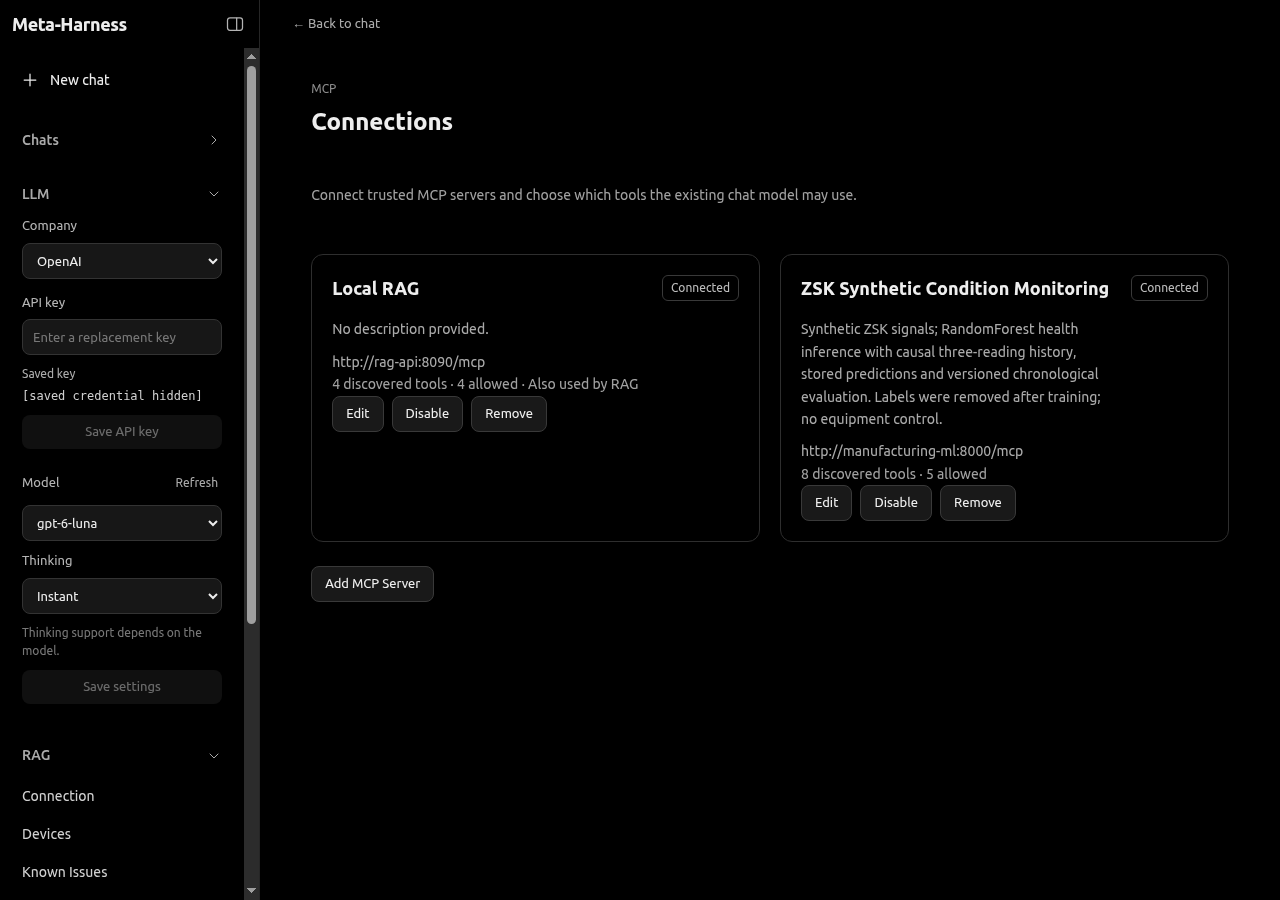
\includegraphics[width=.94\linewidth,trim=310bp 345bp 40bp 250bp,clip]{screenshots/connections.png}\captionof{figure}{Detail from a genuine repository capture of connected RAG/ZSK profiles (9 October 2026). Saved credential metadata was hidden in the supplied publication capture.}\end{center}


\clearpage\chapter{Operating the Decision-Support System}
\section{A short operator workflow}
\begin{enumerate}
\item Identify the line in \textbf{RAG > Devices}; the UI has no dedicated manufacturing-line selector. State dataset code \texttt{ZSK-SIM-01} explicitly and resolve its relationship to RAG \texttt{ZSK-001} before combined analysis.
\item Ask chat to retrieve recent stored measurements and previous comparable recipe conditions. Check timestamps/units; September synthetic readings are not current October telemetry.
\item Request analysis/prediction. Review label, probability, history/warmup and model version; a Healthy label is not an operating-safety clearance.
\item Inspect supporting passages in \textbf{RAG > Knowledge Search} and document/chunk details in \textbf{Documents}. Ranking is not confidence. Chat \textbf{+} attachments are local files, not searchable RAG ingestion.
\item Ask for observations, model result, source evidence, interpretation, inspection priority and uncertainty separately. Treat possible causes as hypotheses.
\item Expand chat tool activity or task \textbf{Requests and outputs}; review the exact call/results. Physical inspections and maintenance decisions remain with the operator and qualified technician.
\end{enumerate}
\section{Example prompts and task recovery}
``What is the current health status of ZSK-001? First verify its dataset identity and data freshness.'' ``Analyze the gearbox vibration trend and explain possible causes using the available documentation.'' ``Compare the latest measurements with previous operating conditions.'' ``What inspection should the operator prioritize based on the available evidence?'' Include the verified dataset code once known; do not instruct the model to guess the mapping.

Check \textbf{Run as task} before Send for durable work, or use \textbf{TASKS > Active Tasks > New task}. Monitor the live card; \textbf{View task details} opens plan, Completion checks, Verification evidence and Tool execution history/Request and result. PAUSED uses \textbf{Resume}; FAILED uses \textbf{Retry}. Resolve pending \textbf{Approve action/Reject action} and \textbf{Reconcile outcome} first. Ordinary chat uses \textbf{Confirm and run/Decline} and \textbf{Retry response}. Cancellation preserves past effects. ``100\% verified'' means task predicates passed; response-only completion explicitly verifies no external operation. Scheduled Tasks supports cron/one-time execution; there is no trigger control.
\begin{center}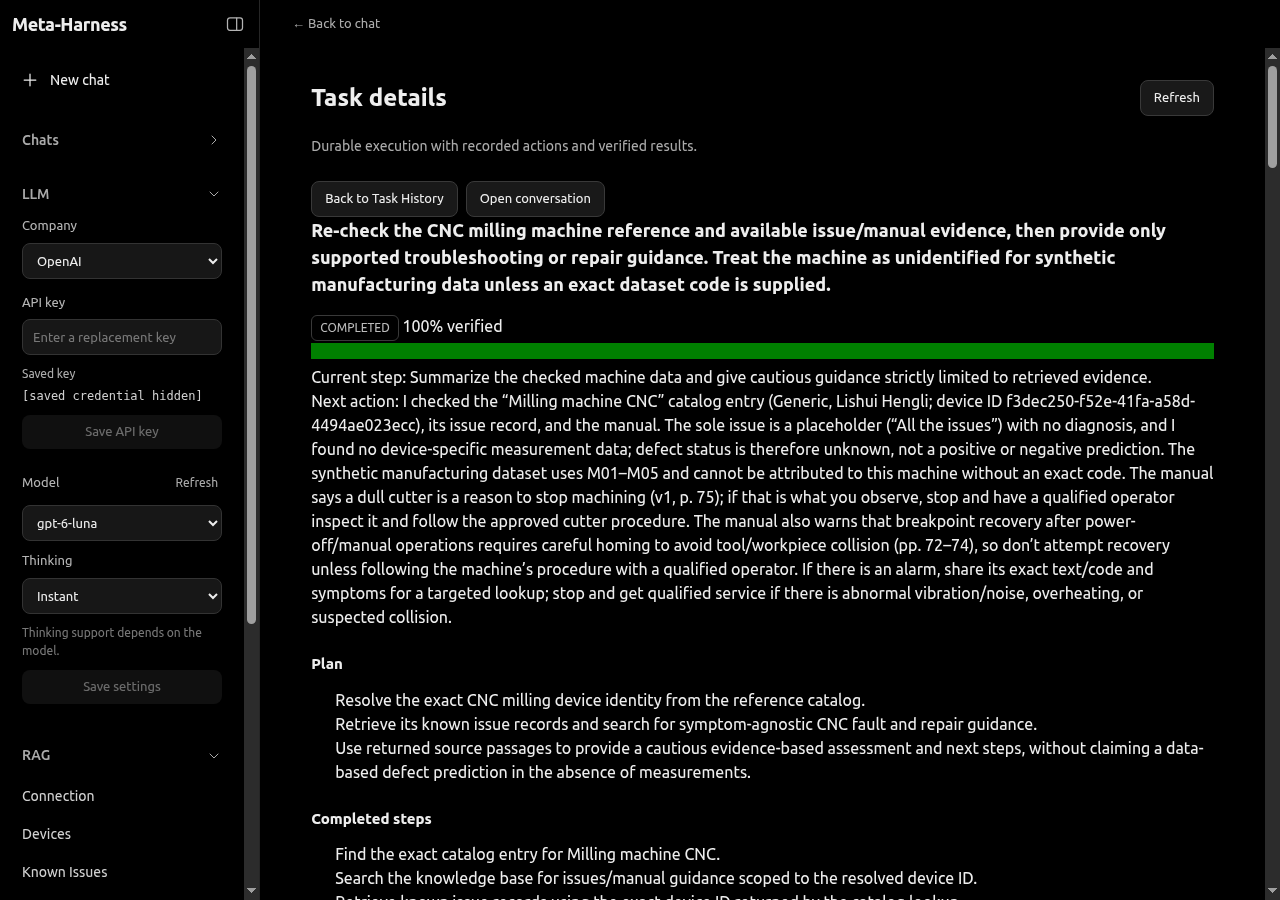
\includegraphics[width=.94\linewidth,trim=300bp 510bp 45bp 85bp,clip]{screenshots/task-details.png}\captionof{figure}{Detail from a genuine task-detail capture. This recorded CNC example illustrates the actual controls, not a ZSK diagnosis; its verified predicates do not certify industrial correctness.}\end{center}
\source{\path{ui/src/components/tasks/tasks-workspace.tsx}; \path{ui/src/components/chat/task-feedback.tsx}; \path{ui/src/components/rag/management.tsx}; \path{ui/src/App.tsx}; service READMEs and \path{docs/OPERATIONS.md}.}

\clearpage\renewcommand{\bibname}{References}\addcontentsline{toc}{chapter}{References}\begingroup\small\setlength{\parskip}{2pt}\bibliographystyle{unsrt}\bibliography{references}\endgroup\end{document}